% !TeX program = lualatex
% !TeX root = ../../main.tex
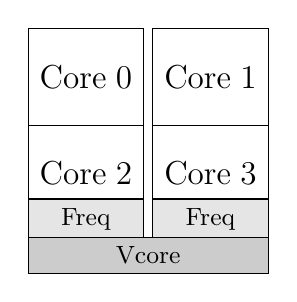
\begin{tikzpicture}[every node/.style={text centered}]
	\draw 	(0, -1.5em)		node[rectangle, draw, text width=3.5em, minimum height=3.5em]
				{\large{Core 0}}

			(4.5em, -1.5em)		node[rectangle, draw, text width=3.5em, minimum height=3.5em]
				{\large{Core 1}}

			(0, -5em)		node[rectangle, draw, text width=3.5em, minimum height=3.5em]
				{\large{Core 2}}
			(0, -6.65em)	node[rectangle, draw, text width=3.5em, minimum height=1.3em, fill=gray!20]
				{\small{Freq}}

			(4.5em, -5em)		node[rectangle, draw, text width=3.5em, minimum height=3.5em]
				{\large{Core 3}}
			(4.5em, -6.65em)	node[rectangle, draw, text width=3.5em, minimum height=1.3em, fill=gray!20]
				{\small{Freq}}
			(2.25em, -7.95em)	node[rectangle, draw, text width=8em, minimum height=1.3em, fill=gray!40]
				{\small{Vcore}}
;
\end{tikzpicture}